%%%% Below from simulation.tex on Sep 16 2020 %%%%
\begin{table}[tp]
	\centering
\caption{Performance improvement of \slearn over \primarybase when the number of pilot
  tasks is varied.
  % {Percentile average task waiting times are calculated after removing thin jobs.}
}
\label{table:sim:numPilots:2STrace}
\vspace{-0.25in}
{\small	
	%\begin{tabular}{cccccccc}
		%\begin{tabular}{cp{0.18in}|p{0.18in}|p{0.18in}|p{0.18in}|p{0.18in}|p{0.18in}|p{0.18in}}
		\begin{tabular}{cp{0.18in}p{0.18in}p{0.18in}p{0.18in}p{0.18in}p{0.18in}p{0.18in}}
		\\ 
% \Xhline{3\arrayrulewidth}
\hline
			 & \multicolumn{7}{c}{Fraction of tasks chosen as pilot tasks}\\
		 &1\%&2\%&5\%&10\%&15\%&20\%&25\%\\  
			    	%Avg. error &X.XXx\%&6.14\%&5.42\%&4.94\%&5.53\%&4.25\%&4.15\%&2.9\%                                    \\
\hline
			& \multicolumn{7}{c}{2STrace \updated{2S - 12th May 2020}}\\
\hline
		     	%P50 pred. error \hspace{-0.1in}&19.01\%&18.23\%&14.04\%&11.80\%&10.94\%&9.46\%&8.39\%                                    \\
			%Avg. JCT speedup \hspace{-0.1in}&1.14&1.14&1.44x&1.38x&1.29x&1.23x&1.17x \\
			%P50 speedup\hspace{-0.1in}&1.28&1.29&1.44x&1.36x&1.31x&1.28x&1.21x  \\
			P50 pred. error (\%) \hspace{-0.1in}&19.35&18.98&18.45&16.95&15.23&14.22&13.32\\
			Avg. JCT speedup ($\times$)\hspace{-0.1in}&1.24&1.23&1.27&1.28&1.21&1.15&1.08  \\
			P50 speedup ($\times$)\hspace{-0.1in}&0.92&0.92&0.94&0.95&0.90&0.84&0.79\\
	      		
			%Avg. job waiting time (KSec) &3882.04&4050.95&4450.96&4524.77&4791.99                                    \\
	      		%P50 avg. waiting time (KSec) &4.66&4.31&4.78&5.41&7.33                                    \\
	      		%P70 avg. waiting time (KSec) &79.02&91.62&107.55&151.72&201.46                                    \\
	      		%P90 avg. waiting time (KSec) &340.62&329.98&315.87&309.55&299.73                                    \\
			
\hline
			& \multicolumn{7}{c}{GTrace \updated{G11 - 9th July 2020}}\\
\hline
		P50 pred. error (\%)\hspace{-0.1in}&10.17&10.09&8.33&5.28&5.35&4.80&4.09\\
		Avg. JCT speedup ($\times$)\hspace{-0.1in}&1.41&1.40&1.43&1.13&0.90&0.76&0.63\\
		P50 speedup ($\times$)\hspace{-0.1in}&1.12&1.12&1.10&1.07&1.02&1.0&0.94\\
		%P50 pred. error \hspace{-0.1in}&8.90\%&8.56\%&7.85\%&6.09\%&4.88\%&4.27\%&3.56\%                                    \\
		%Avg. JCT speedup \hspace{-0.1in}&1.34&1.30&1.40x&1.36x&0.98x&0.84x&0.72x  \\
		%P50 speedup\hspace{-0.1in}&0.86&0.87&0.74x&0.70x&0.73x&0.68x&0.73x \\
\hline
			& \multicolumn{7}{c}{GTrace19 \updated{G19 - 26th Aug 2020}}\\
\hline
		P50 pred. error (\%)\hspace{-0.1in}&56.44&55.64&48.35&43.15&39.39&37.08&33.54\\
		Avg. JCT speedup ($\times$)\hspace{-0.1in}&1.24&1.23&1.18&1.10&0.99&0.92&0.84\\
		P50 speedup ($\times$)\hspace{-0.1in}&1.46&1.30&1.06&0.97&0.84&0.81&0.73\\
\hline
	\end{tabular}
}
\vspace{-0.1in}
\end{table}






\if 0
\begin{table}
\caption{Fraction of overestimated jobs and incorrect queue placement for 2STrace. Job performance in the third column is relative to the \oracle. \updated{2S - 14th June 2020}}
  \label{table:sim:overestimatedJobs}
\vspace{-0.1in}	
  \centering
      {\small
	\begin{tabular}{|c|c|c|c|c|} 
	  \hline
		& Overestima- & Misplaced over- & Slowed misp- & Average (P50)\\
		& ted jobs & estimated jobs & laced jobs & Positive error\\
	  \hline
		%\primarybase & 59.37\% & 36.02\% & 82.84\% \\
		\primarybase & 59.37\% & 21.09\% & 17.72\% & 1253.60 (66.38)\% \\
	  \hline
	  	%\slearn & 43.75\% & 8.09 \% & 100\% \\
	  	\slearn & 43.75\% & 2.87 \% & 2.63\% & 29.64 (17.79)\% \\
	  \hline
	\end{tabular}
      }
\vspace{-0.1in}	
\end{table}

\begin{table}
\caption{Fraction of underestimated jobs and incorrect queue placement for 2STrace. Job performance in the third column is relative to the \oracle. \updated{2S - 14th June 2020}}
  \label{table:sim:underestimatedJobs}
\vspace{-0.1in}	
  \centering
      {\small
	\begin{tabular}{|c|c|c|c|c|} 
	  \hline
		& Underestim- & Misplaced under & Spedup misp- & Average (P50)\\
		& ated jobs & estimated jobs & laced jobs & Negative error\\
	  \hline
		%\primarybase & 40.63\% & 25.15\% & 82.81\% \\
		\primarybase & 40.63\% & 10.22\% & 8.46\% & -39.33 (-31.59)\%\\
	  \hline
	  	%\slearn & 55.45\% & 12.77 \% & 45.83\% \\
	  	\slearn & 55.45\% & 5.75 \% & 2.63\% & -26.13 (-19.61)\% \\
	  \hline
	\end{tabular}
      }
\vspace{-0.1in}	
\end{table}
\fi


%%%% Above from simulation.tex on Sep 16 2020 %%%%



%%%% Below from simulation.tex on Sep 17 2020 %%%%
\if 0
\begin{table*}[tp]
	\centering
\caption{Performance improvement of \slearn over \primarybase for GTrace when the number of pilot
  tasks is varied.
  % {Percentile average task waiting times are calculated after removing thin jobs.}
}
\label{table:sim:numPilots:GTrace}
\vspace{-0.25in}
{\small	
	\begin{tabular}{cccccccc}
		%\caption{GTrace}
		\\ \Xhline{3\arrayrulewidth}
			 & \multicolumn{7}{c}{Fraction of tasks chosen as pilot tasks}      \\
		&1\%&2\%&5\%&10\%&15\%&20\%&25\%	\\  \Xhline{3\arrayrulewidth}
		P50 pred. error \hspace{-0.1in}&8.90\%&8.56\%&7.85\%&6.09\%&4.88\%&4.27\%&3.56\%                                    \\
		Avg. JCT speedup \hspace{-0.1in}&1.34&1.30&1.40x&1.36x&0.98x&0.84x&0.72x  \\
		P50 speedup\hspace{-0.1in}&0.86&0.87&0.74x&0.70x&0.73x&0.68x&0.73x \\
\hline
	\end{tabular}
}
\vspace{-0.1in}
\end{table*}
\fi


%  The two test traces have 1000 jobs each, are 2.25 and 2.15 hours long,
%  respectively, and retain the same job arrival time distribution
%  as the original traces.


\if 0
\begin{figure*}[tp]
\centering
	\subfigure[CDF of normalized task waiting times for all wide jobs]{
	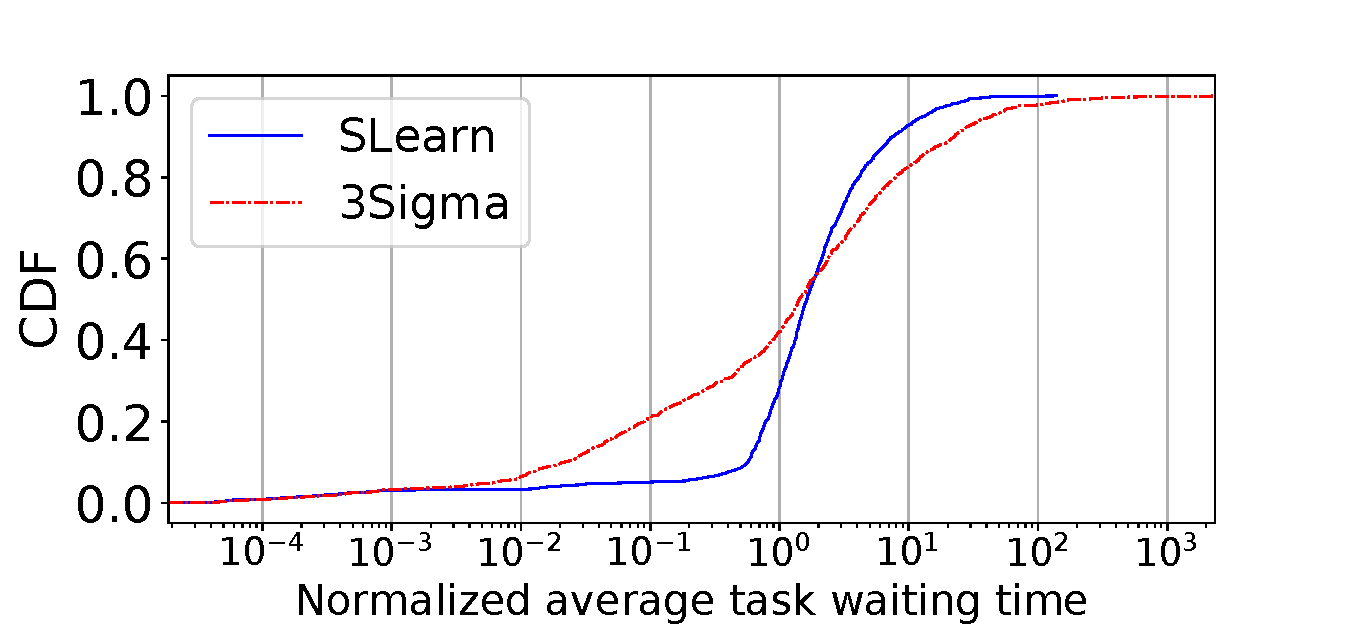
\includegraphics[width=0.31\textwidth]{figures/simulation/normalized_average_task_waiting_time_2STrace.pdf}
	\label{fig:sim:waitingTimesTrial:2STrace:cdf}
	\vspace{-0.1in}
}
	\subfigure[CDF of average waiting times for all wide jobs]{
\vspace{-0.2in}
	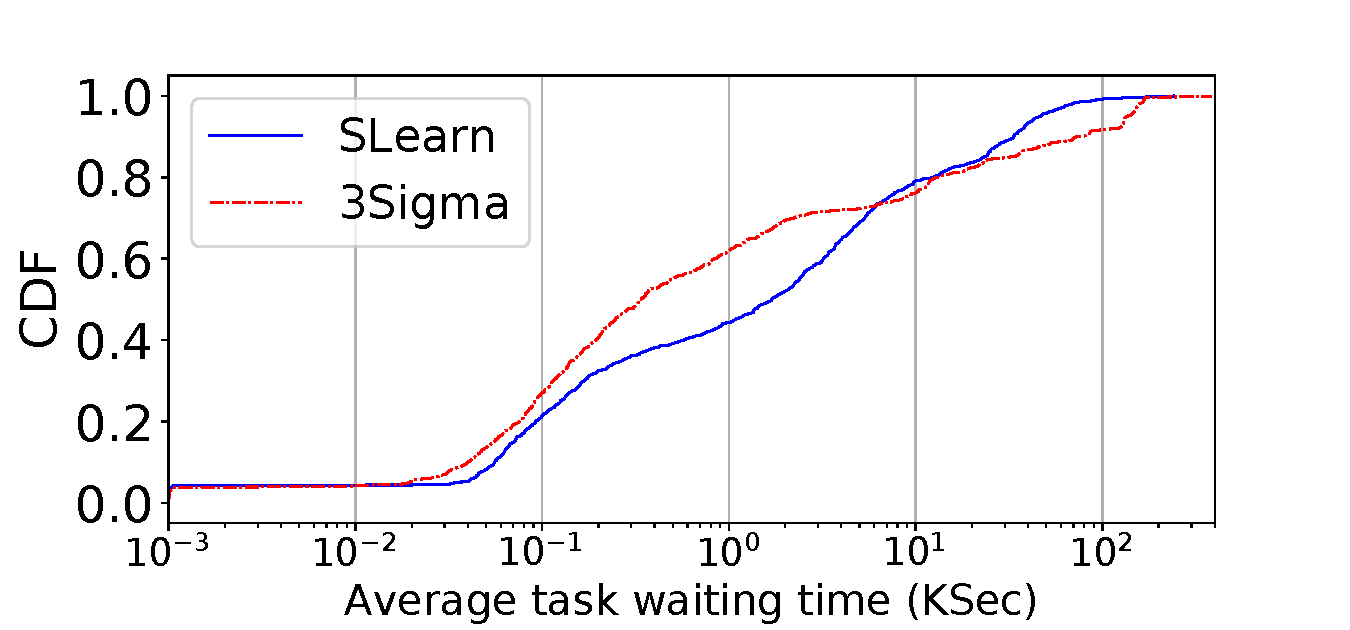
\includegraphics[width=0.31\textwidth]{figures/simulation/average_task_waiting_time_2STrace.pdf}
	%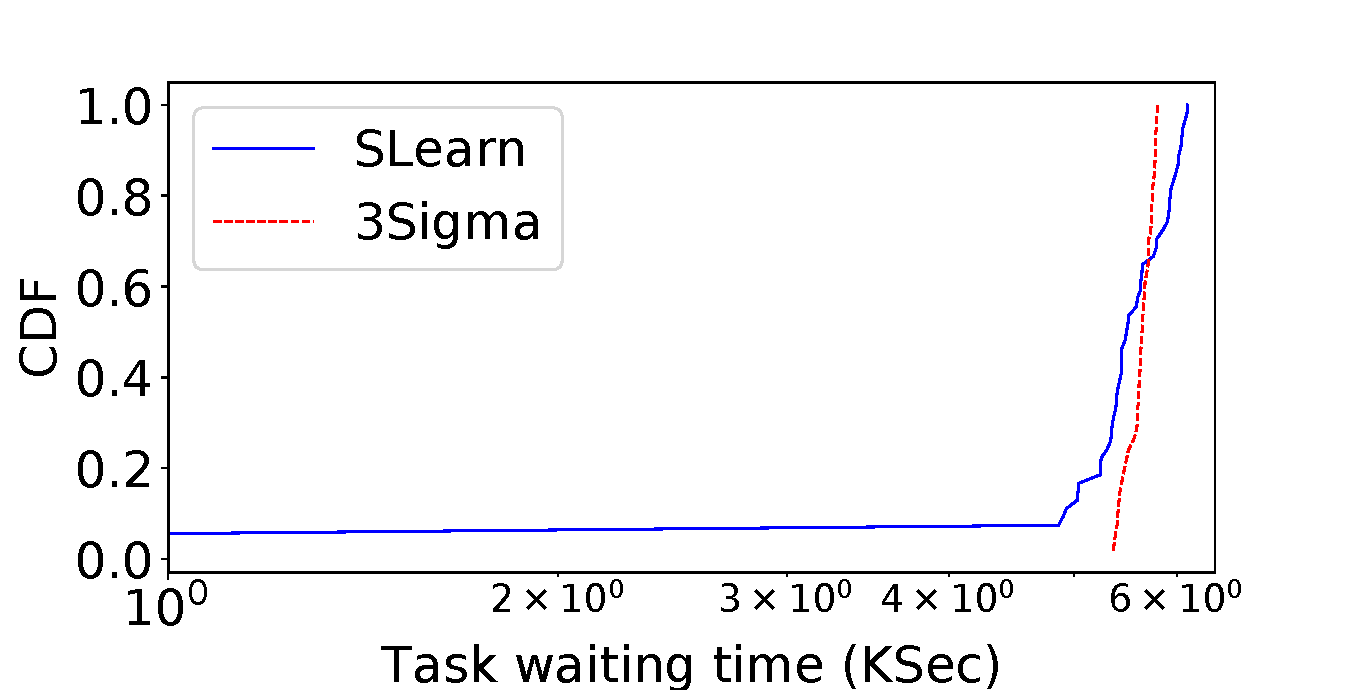
\includegraphics[width=0.31\textwidth]{figures/simulation/task_waiting_time_cdf_JOB-181.pdf}
	\label{fig:sim:waitingTimesTrial:2STrace:same}
	\vspace{-0.1in}
}
	\subfigure[CDF of ratio of waiting times for all wide jobs]{
	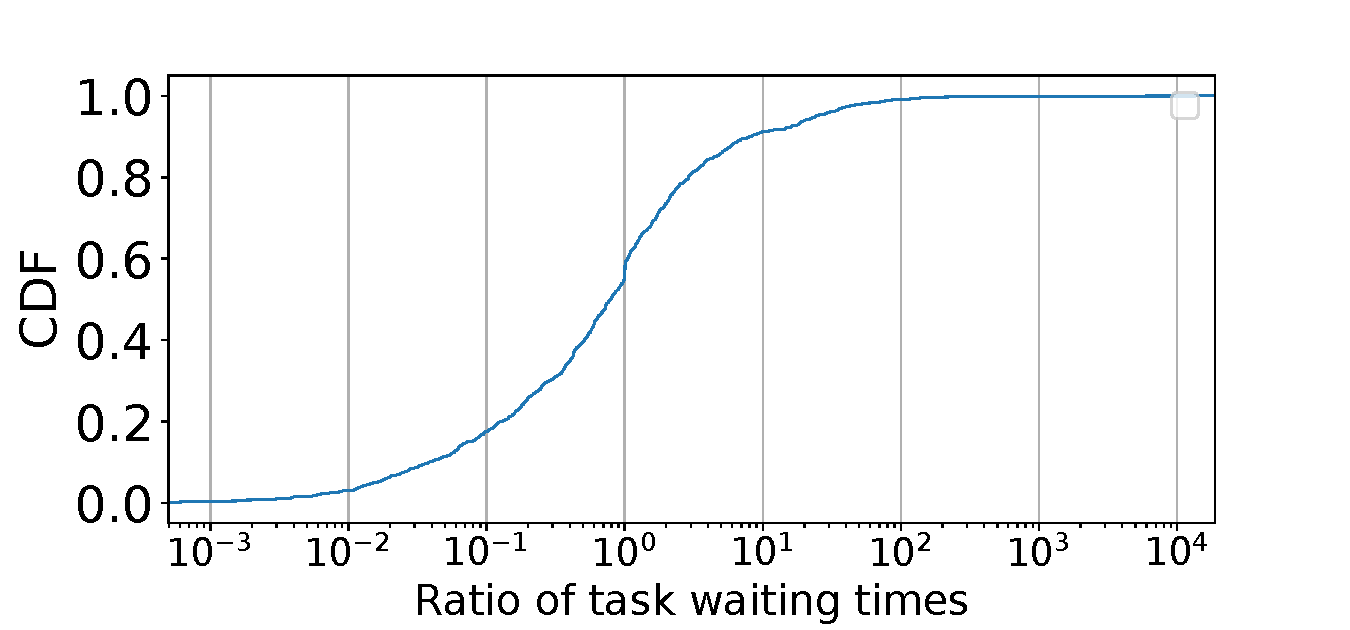
\includegraphics[width=0.31\textwidth]{figures/simulation/ratio_task_waiting_time_2STrace.pdf}
	%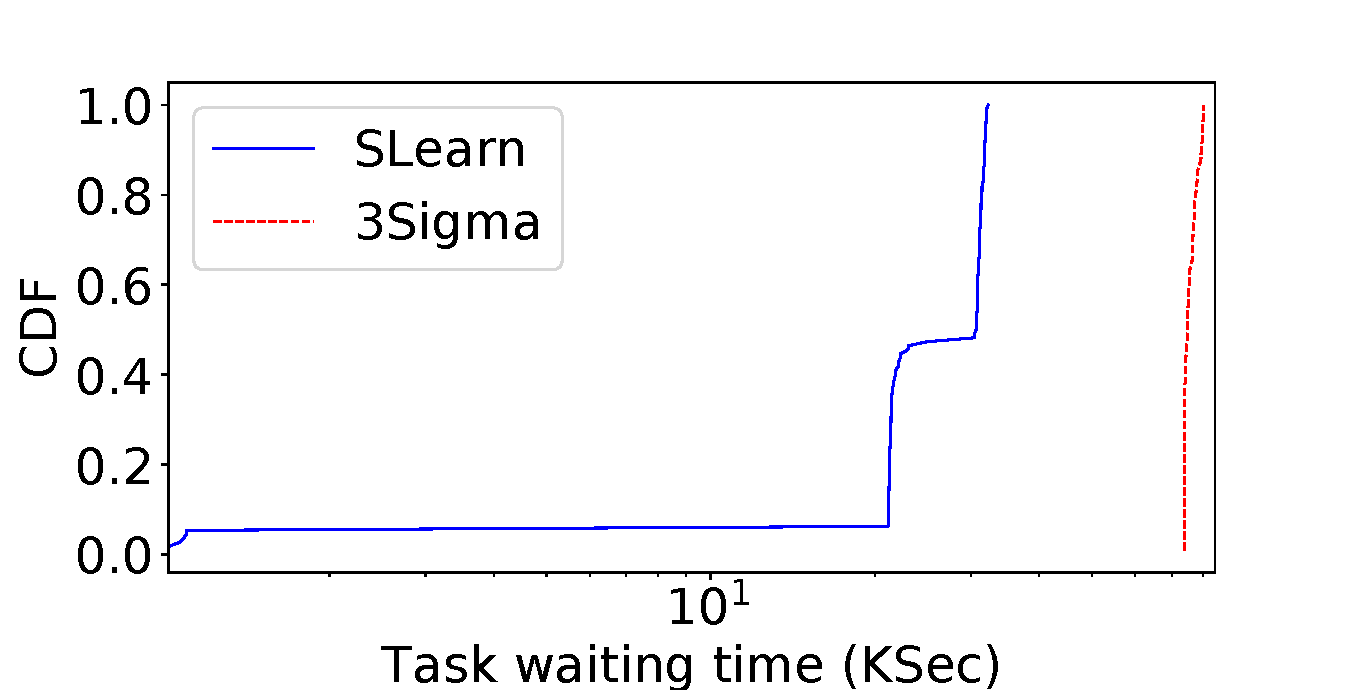
\includegraphics[width=0.31\textwidth]{figures/simulation/task_waiting_time_cdf_JOB-781.pdf}
	\label{fig:sim:waitingTimesTrial:2STrace:improvement}
	\vspace{-0.1in}
}
\vspace{-0.2in}
\caption{Waiting times for jobs in 2STrace - \updated{2S - 12th May 2020}}
\label{fig:sim:waitingTimesTrial}
\vspace{-0.1in}
\end{figure*}
\questionaj{Refer to fig \ref{fig:sim:waitingTimesTrial} and finalize one among the three variants for task waiting time CDF.}
\fi

%%%% Above from simulation.tex on Sep 17 2020 %%%%
